\documentclass{article}
\usepackage{amsmath}
\usepackage{amssymb}
\usepackage{tikz}

\begin{document}

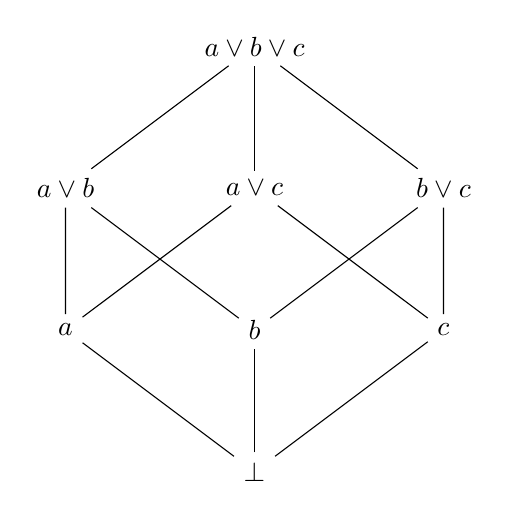
\begin{tikzpicture}[scale=1.2] %, every node/.style={circle,draw,inner sep=1pt}]

\tikzset{
  lattice node/.style={
    inner sep=1pt,
    outer sep=1pt,
  }
}


  % Level 0
  \node (0) at (0,0) {$\bot$};

  % Level 1
  \node (a) at (-2,1.5) {$a$};
  \node (b) at (0,1.5)  {$b$};
  \node (c) at (2,1.5)  {$c$};

  % Level 2
  \node (ab) at (-2,3) {$a \vee b$};
  \node (ac) at (0,3)  {$a \vee c$};
  \node (bc) at (2,3)  {$b \vee c$};

  % Level 3
  \node (abc) at (0,4.5) {$a \vee b \vee c$};

  % Edges
  \draw (0) -- (a);
  \draw (0) -- (b);
  \draw (0) -- (c);

  \draw (a) -- (ab);
  \draw (a) -- (ac);
  \draw (b) -- (ab);
  \draw (b) -- (bc);
  \draw (c) -- (ac);
  \draw (c) -- (bc);

  \draw (ab) -- (abc);
  \draw (ac) -- (abc);
  \draw (bc) -- (abc);
\end{tikzpicture}


\end{document}
